\section{Algorithm}
\label{section: Chapter4/algo}

\begin{figure}[h]
    \centering
    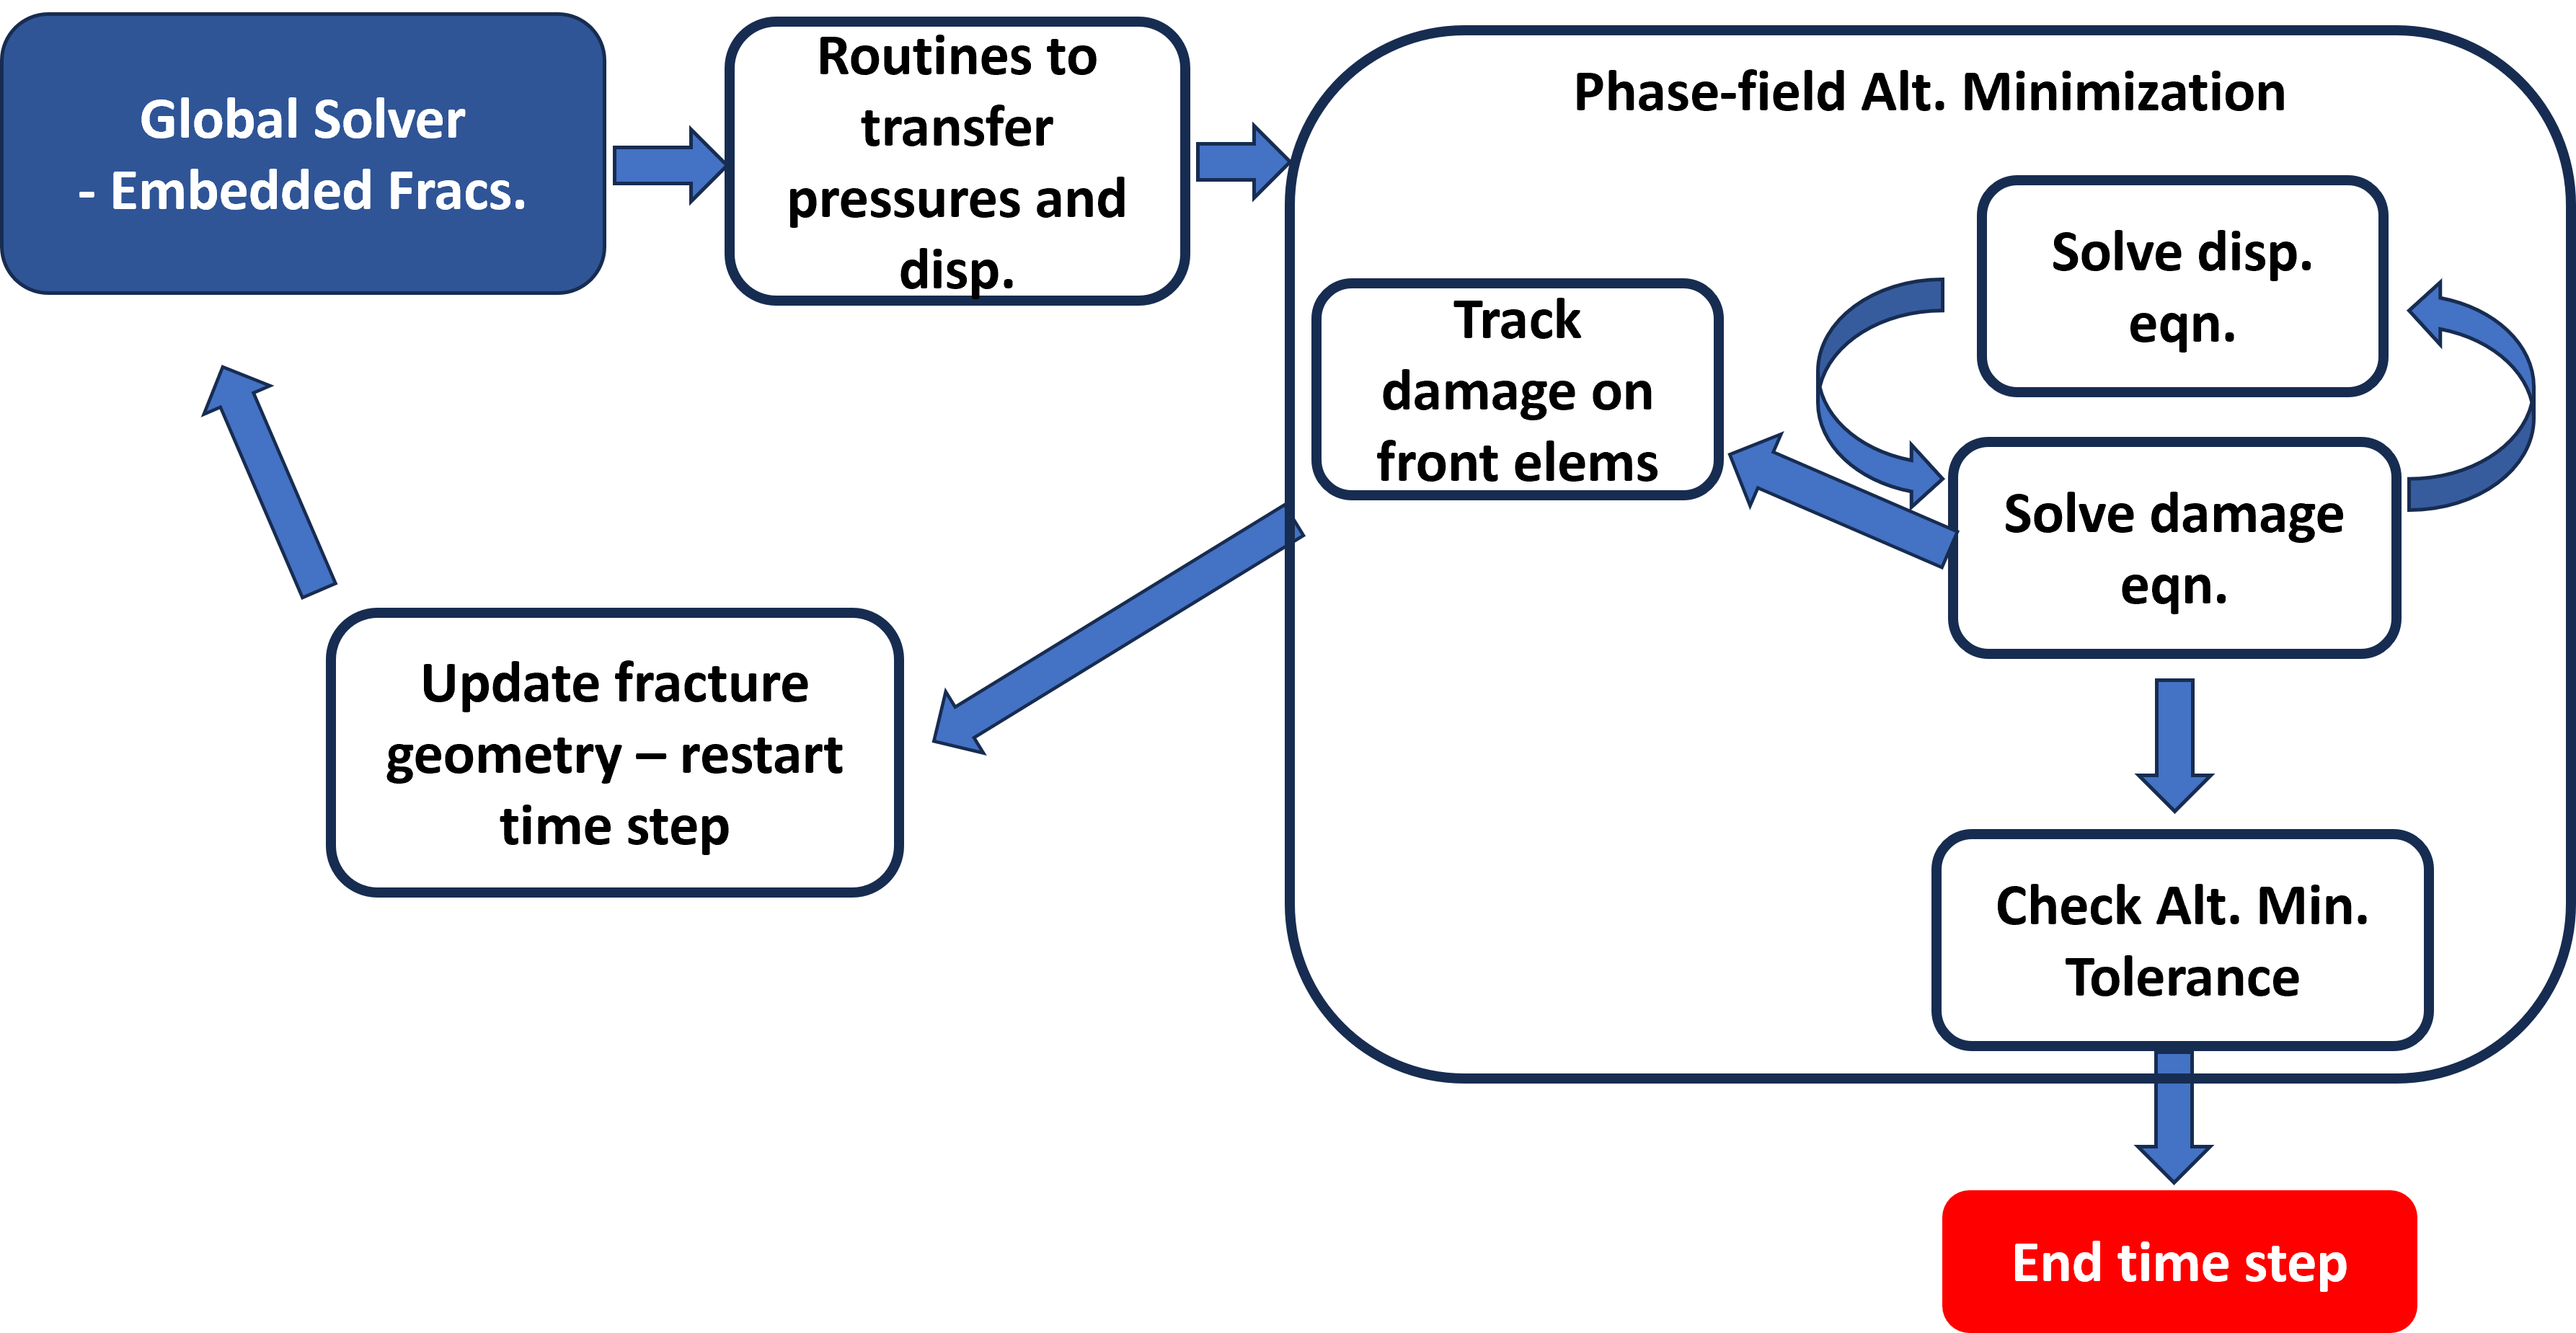
\includegraphics[width=\linewidth]{Chapter4/figures/planar3D_algorithm.png}
    \caption{Multi-resolution solution algorithm.}
    \label{fig:MR_planar_algo}
\end{figure}

A high-level description of the propagation algorithm for planar fractures in 3D is shown in Figure \ref{fig:MR_planar_algo}. It summarizes each of the steps involved in the solution procedure for a single time-setp. The process begins with the solution of the global problem (i.e, the box colored in blue in \ref{fig:MR_planar_algo}). As pointed out in chapter \ref{section: Chapter3}, the algorithm is designed without relying on specific numerical methods for the approximation of the solutions. With the approximate solutions for displacements and pressures, transfer then to the local problem, as explained in the steps (3) and (4) of Algorithm \ref{fig:solution_algorithm}.

In the 2D algorithm, one would now move to the solution of the local problem with an alternate minimization approach and only then check for fracture propagation. In the proposed 3D algorithm, this is changed and a damage tracking function is launched in parallel with the damage solver. This function checks the amount of damage in the elements of the fracture front. Different measurements of damage can be employed, and they will likely depend on the discretization method employed. A simple one, which works well for planar fractures in structured grids is the volume of damage, which is defined as the total volume of subdiscretization' elements with damage above a threshold (usually around 0.9). This works well in this case, since for planar fractures aligned with structured grids, the fracture area on each element can be predicted beforehand. This simpliefied criteria is used in the example problems that will be shown next. For more general discretization types, a more robust approach is to identify the maximum damage level on each of the element faces. 

If any of the front elements is identified as being cracked (i.e, the level of damage on it is very high), the alternate minimization algorithm is stopped and the geometry of the discrete fracture, in the global problem is updated, with a planar cut that conforms with the current fracture being inserted. This process is done for all cracked front elements. The current time-step is then re-launched. This steps are repeated until the alternate minimization algorithm in the local problem converges without triggering the propagation criteria. When this happens, a equilibrium state is obtained and the time-step can be advanced.

\subsection{Fracture front construction}

lorem ipsum lorem ipsum lorem ipsum lorem ipsum lorem ipsum lorem ipsum lorem ipsum lorem ipsum lorem ipsum lorem ipsumlorem ipsum lorem ipsum lorem ipsum lorem ipsum lorem ipsumlorem ipsum lorem ipsum lorem ipsum lorem ipsum lorem ipsumlorem ipsum lorem ipsum lorem ipsum lorem ipsum lorem ipsum Figure \ref{fig:lorem0}.

\begin{figure}[h]
    \centering
    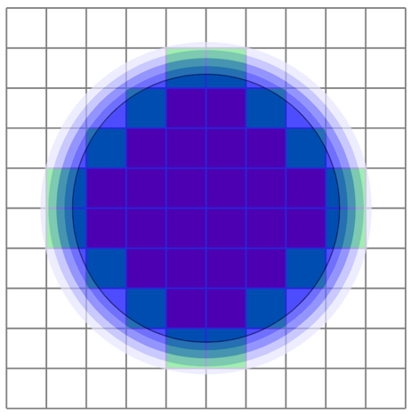
\includegraphics[width=0.5\linewidth]{Chapter4/figures/blue_circle.png}
    \caption{Multi-resolution solution algorithm.}
    \label{fig:lorem0}
\end{figure}

\subsection{Tracking damage in the fracture front elements}

lorem ipsum lorem ipsum lorem ipsum lorem ipsum lorem ipsum lorem ipsum lorem ipsum lorem ipsum lorem ipsum lorem ipsumlorem ipsum lorem ipsum lorem ipsum lorem ipsum lorem ipsumlorem ipsum lorem ipsum lorem ipsum lorem ipsum lorem ipsumlorem ipsum lorem ipsum lorem ipsum lorem ipsum lorem ipsum


% \begin{figure}[h]
%     \centering
%     \begin{subfigure}{.45\textwidth}
%         \centering
%         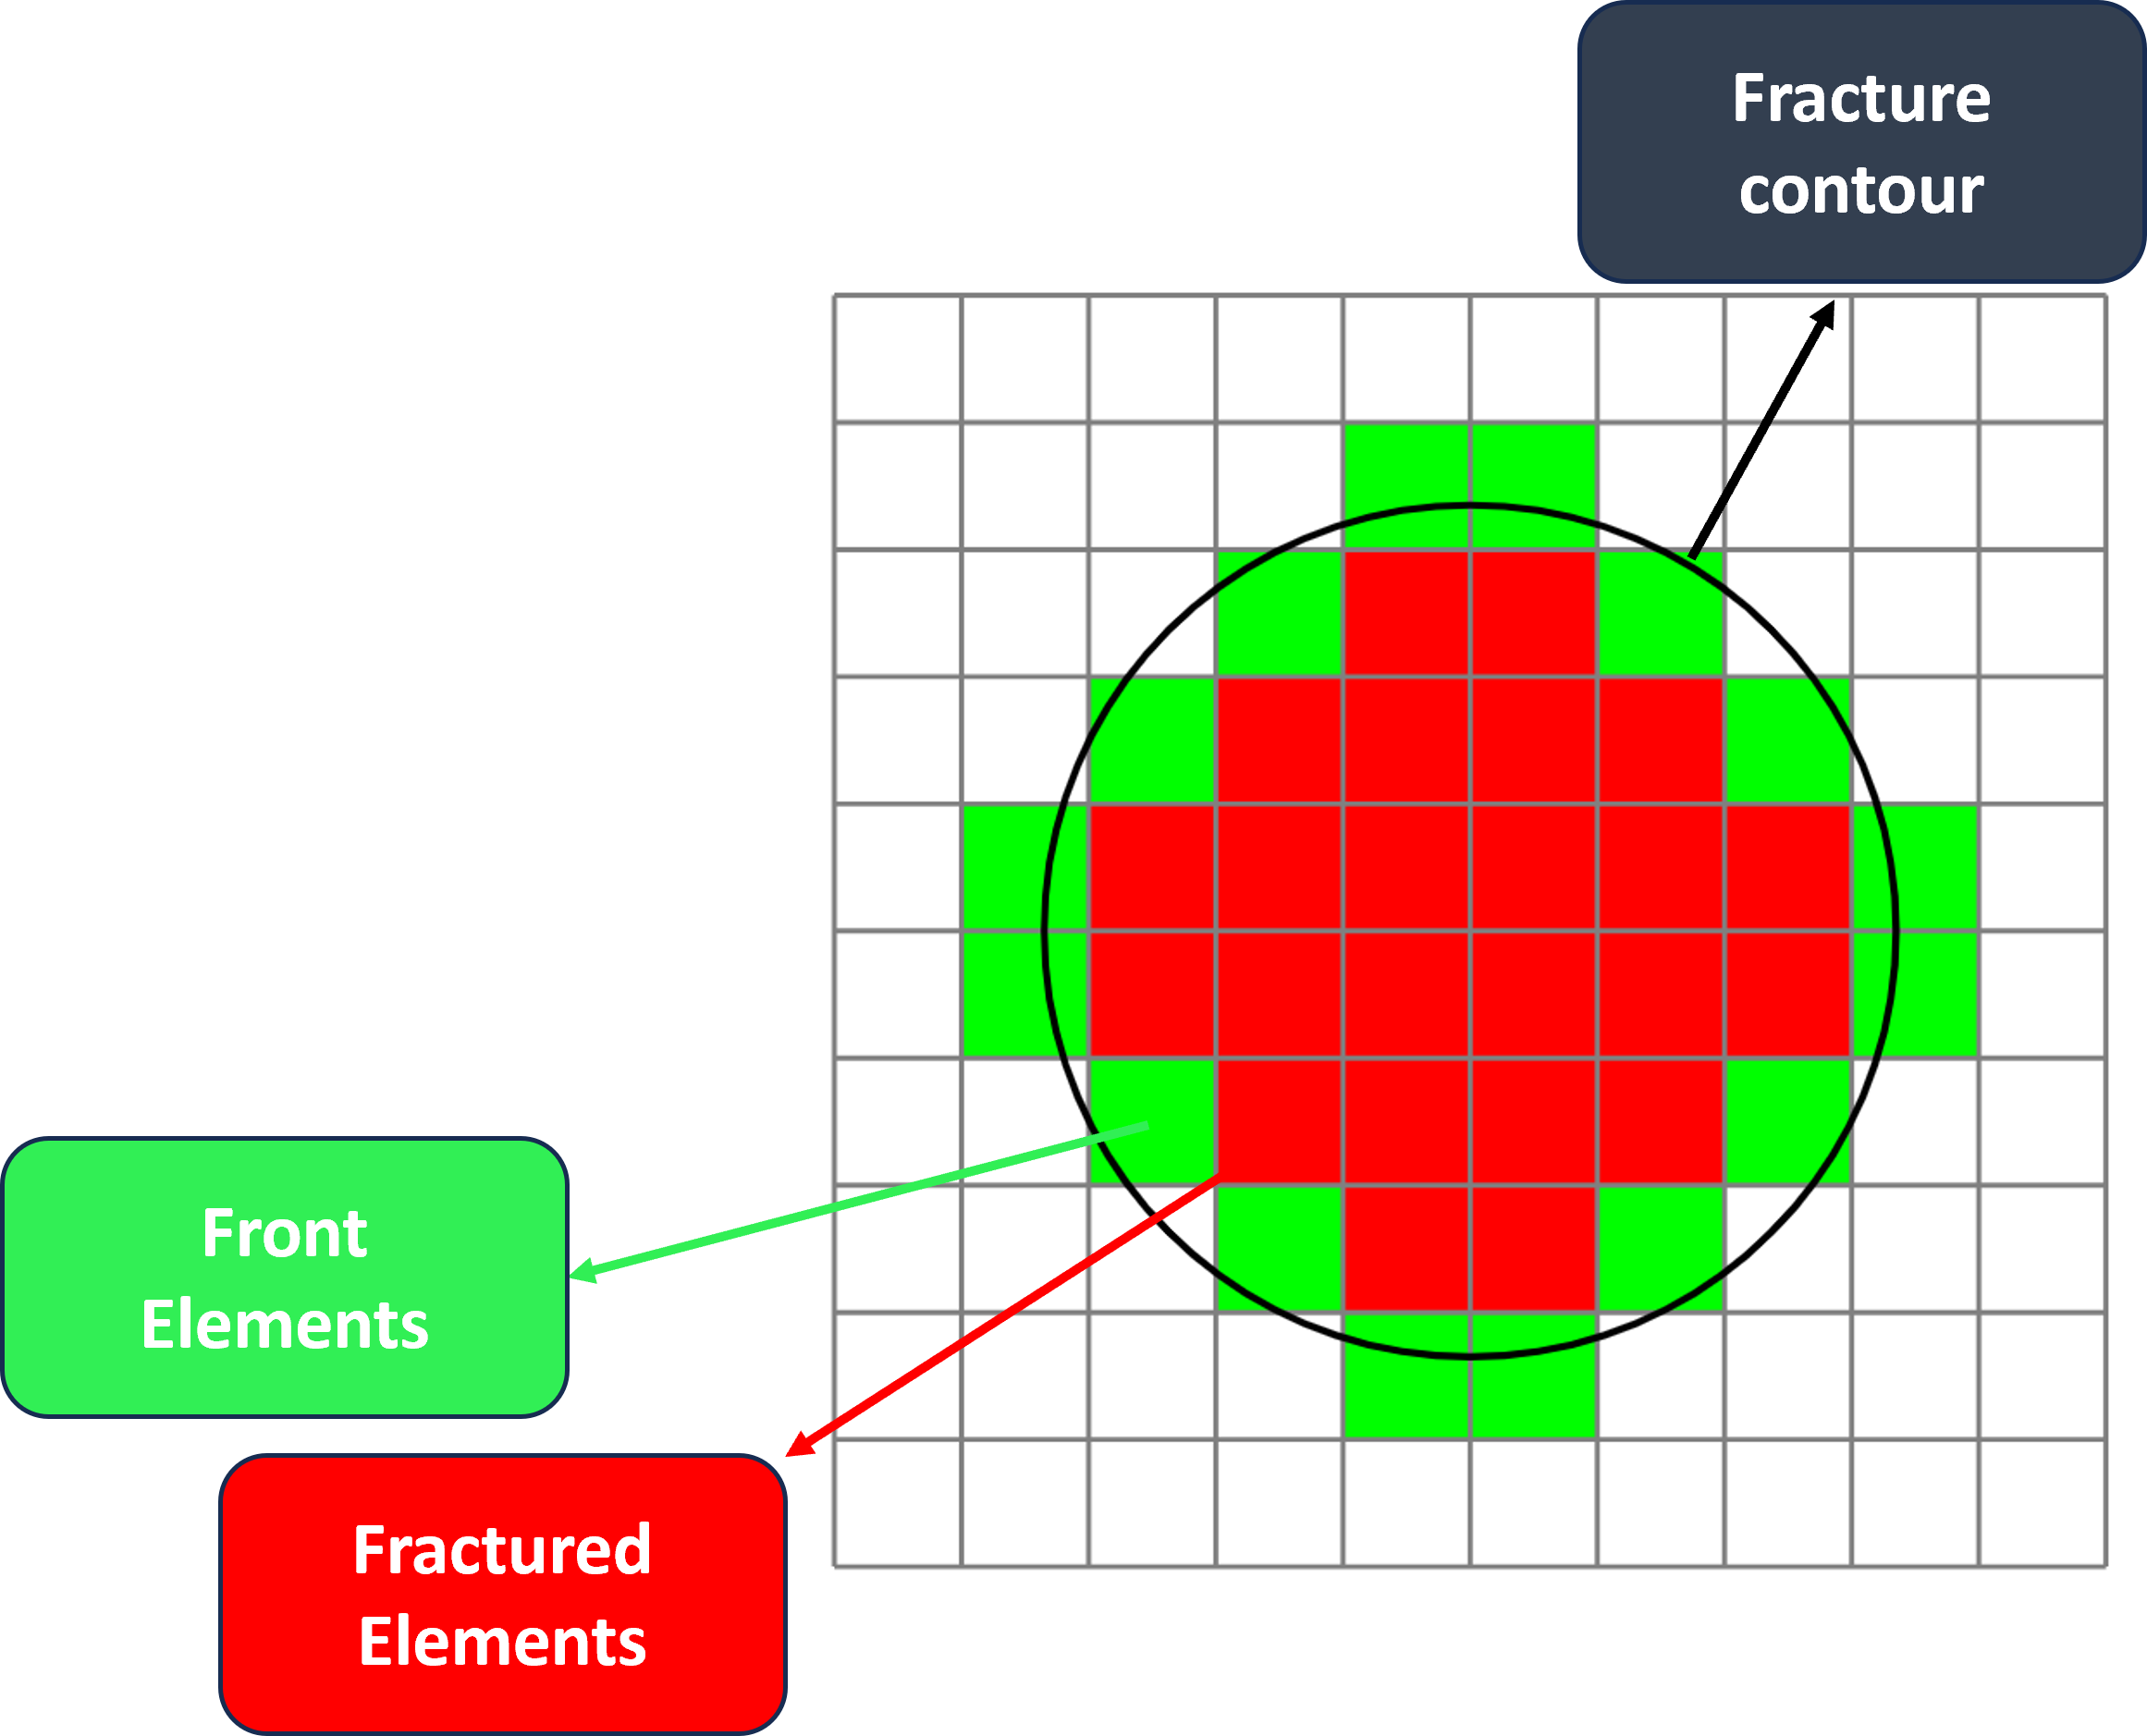
\includegraphics[width=\linewidth]{Chapter4/figures/penny_with_descriptions.png}
%         \caption{Multi-resolution solution algorithm.}
%         \label{fig:lorem1}
%     \end{subfigure}%
%     \begin{subfigure}{.45\textwidth}
%         \centering
%         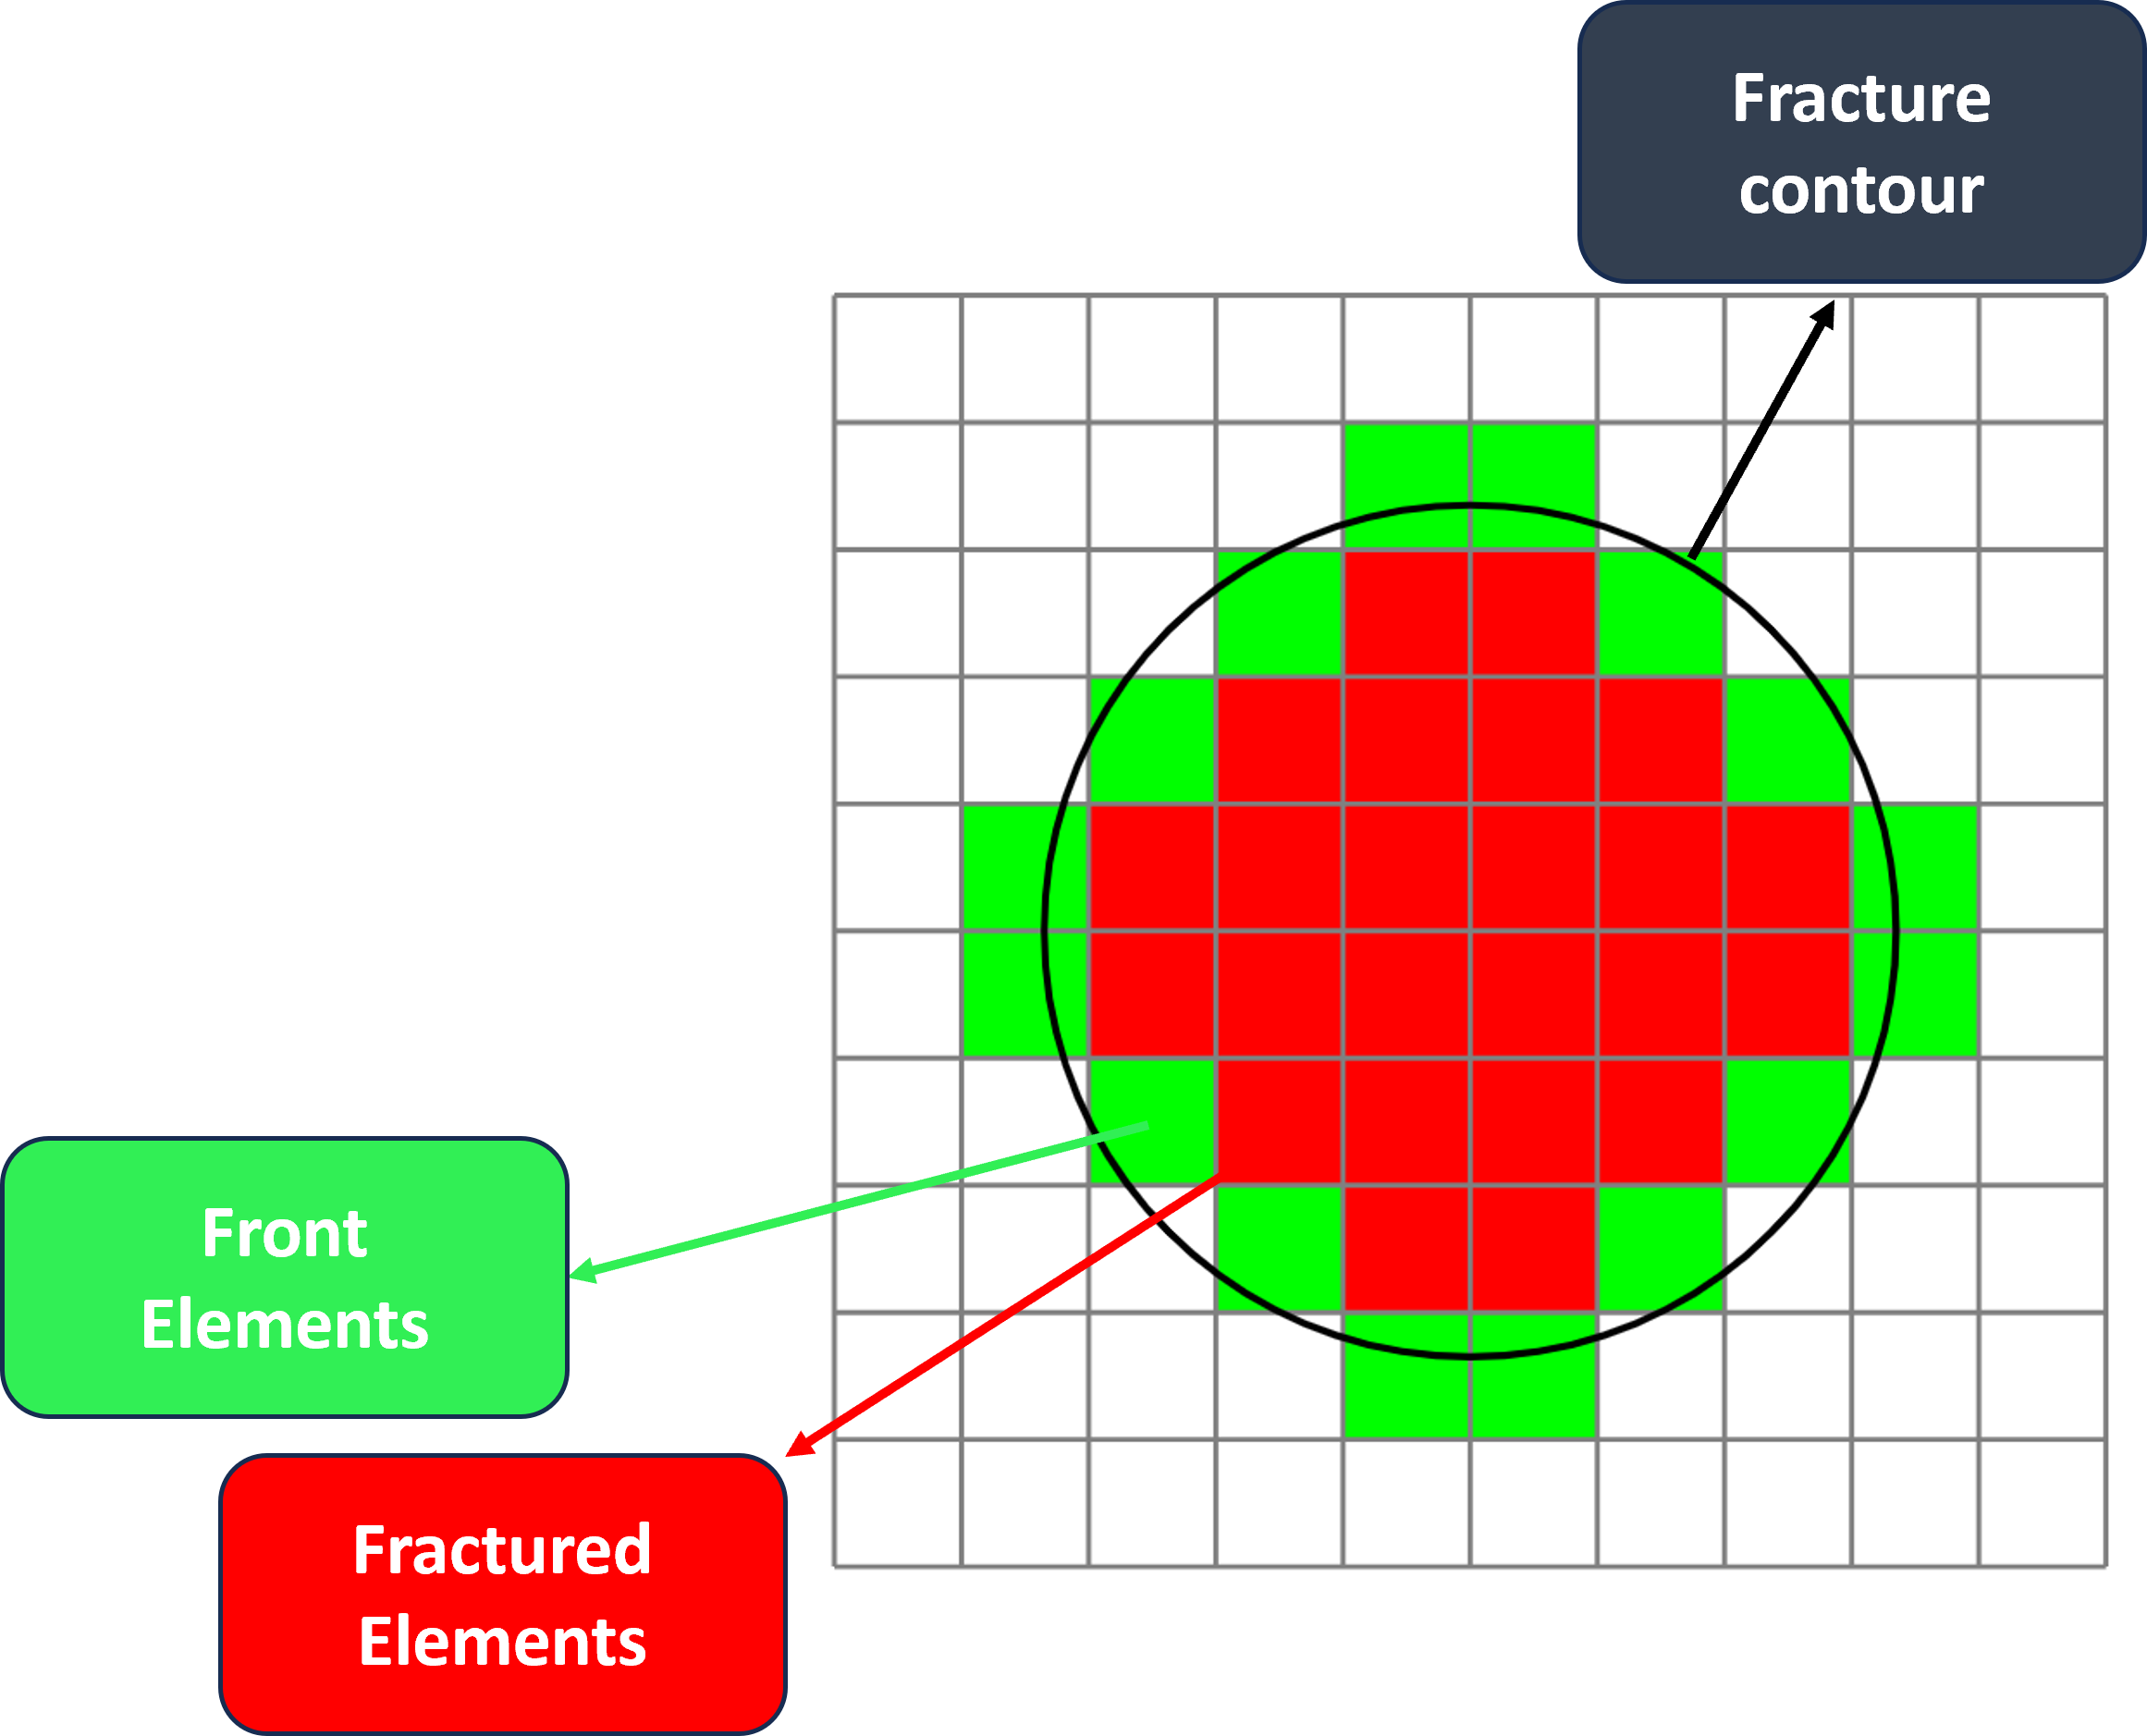
\includegraphics[width=\linewidth]{Chapter4/figures/penny_with_descriptions.png}
%         \caption{Multi-resolution solution algorithm.}
%         \label{fig:lorem2}
%     \end{subfigure}%
    
%     \bigskip
%     \begin{subfigure}{.45\textwidth}
%         \centering
%         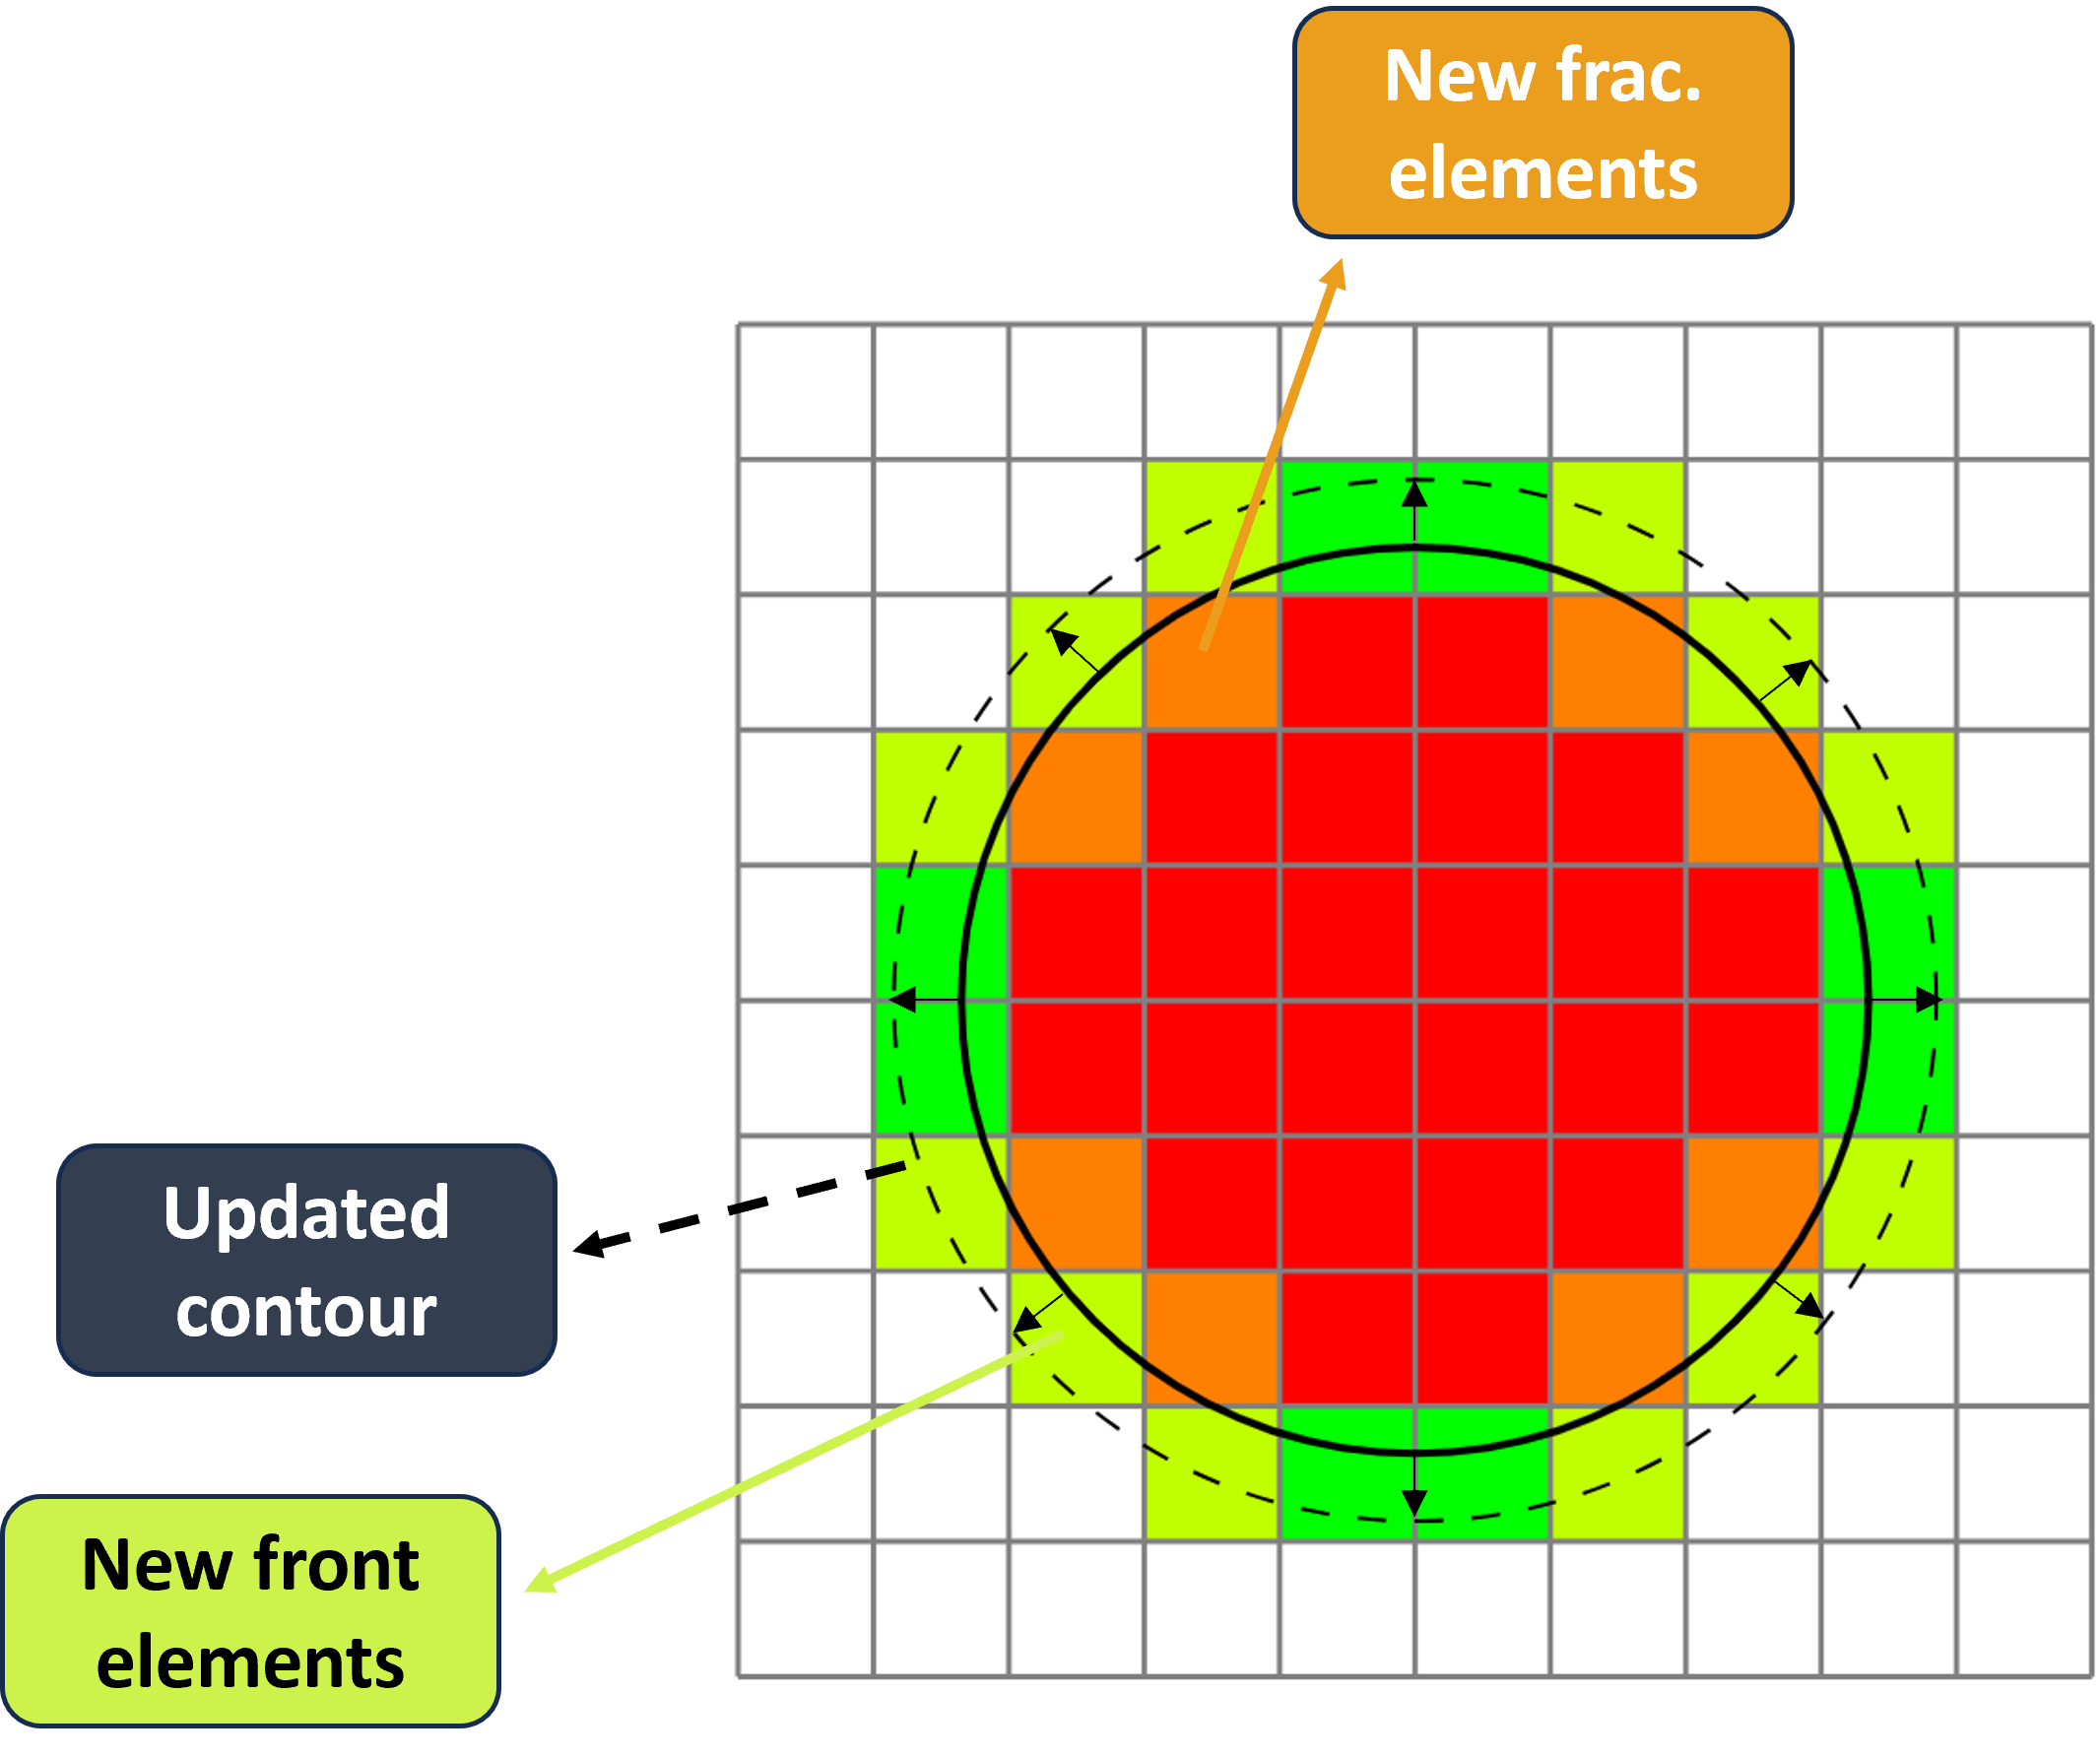
\includegraphics[width=\linewidth]{Chapter4/figures/larger_penny_with_descriptions.png}
%         \caption{Multi-resolution solution algorithm.}
%         \label{fig:lorem3}
%     \end{subfigure}
%     \begin{subfigure}{.45\textwidth}
%         \centering
%         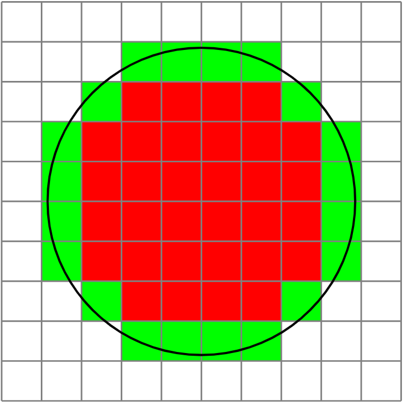
\includegraphics[width=0.65\linewidth]{Chapter4/figures/larger_penny.png}
%         \caption{Multi-resolution solution algorithm.}
%         \label{fig:lorem4}
%     \end{subfigure}
%       \caption{Schematic of propagation steps.}
% \end{figure}

% \begin{figure}[h]
%     \centering
%     \begin{subfigure}{\textwidth}
%         \centering
%         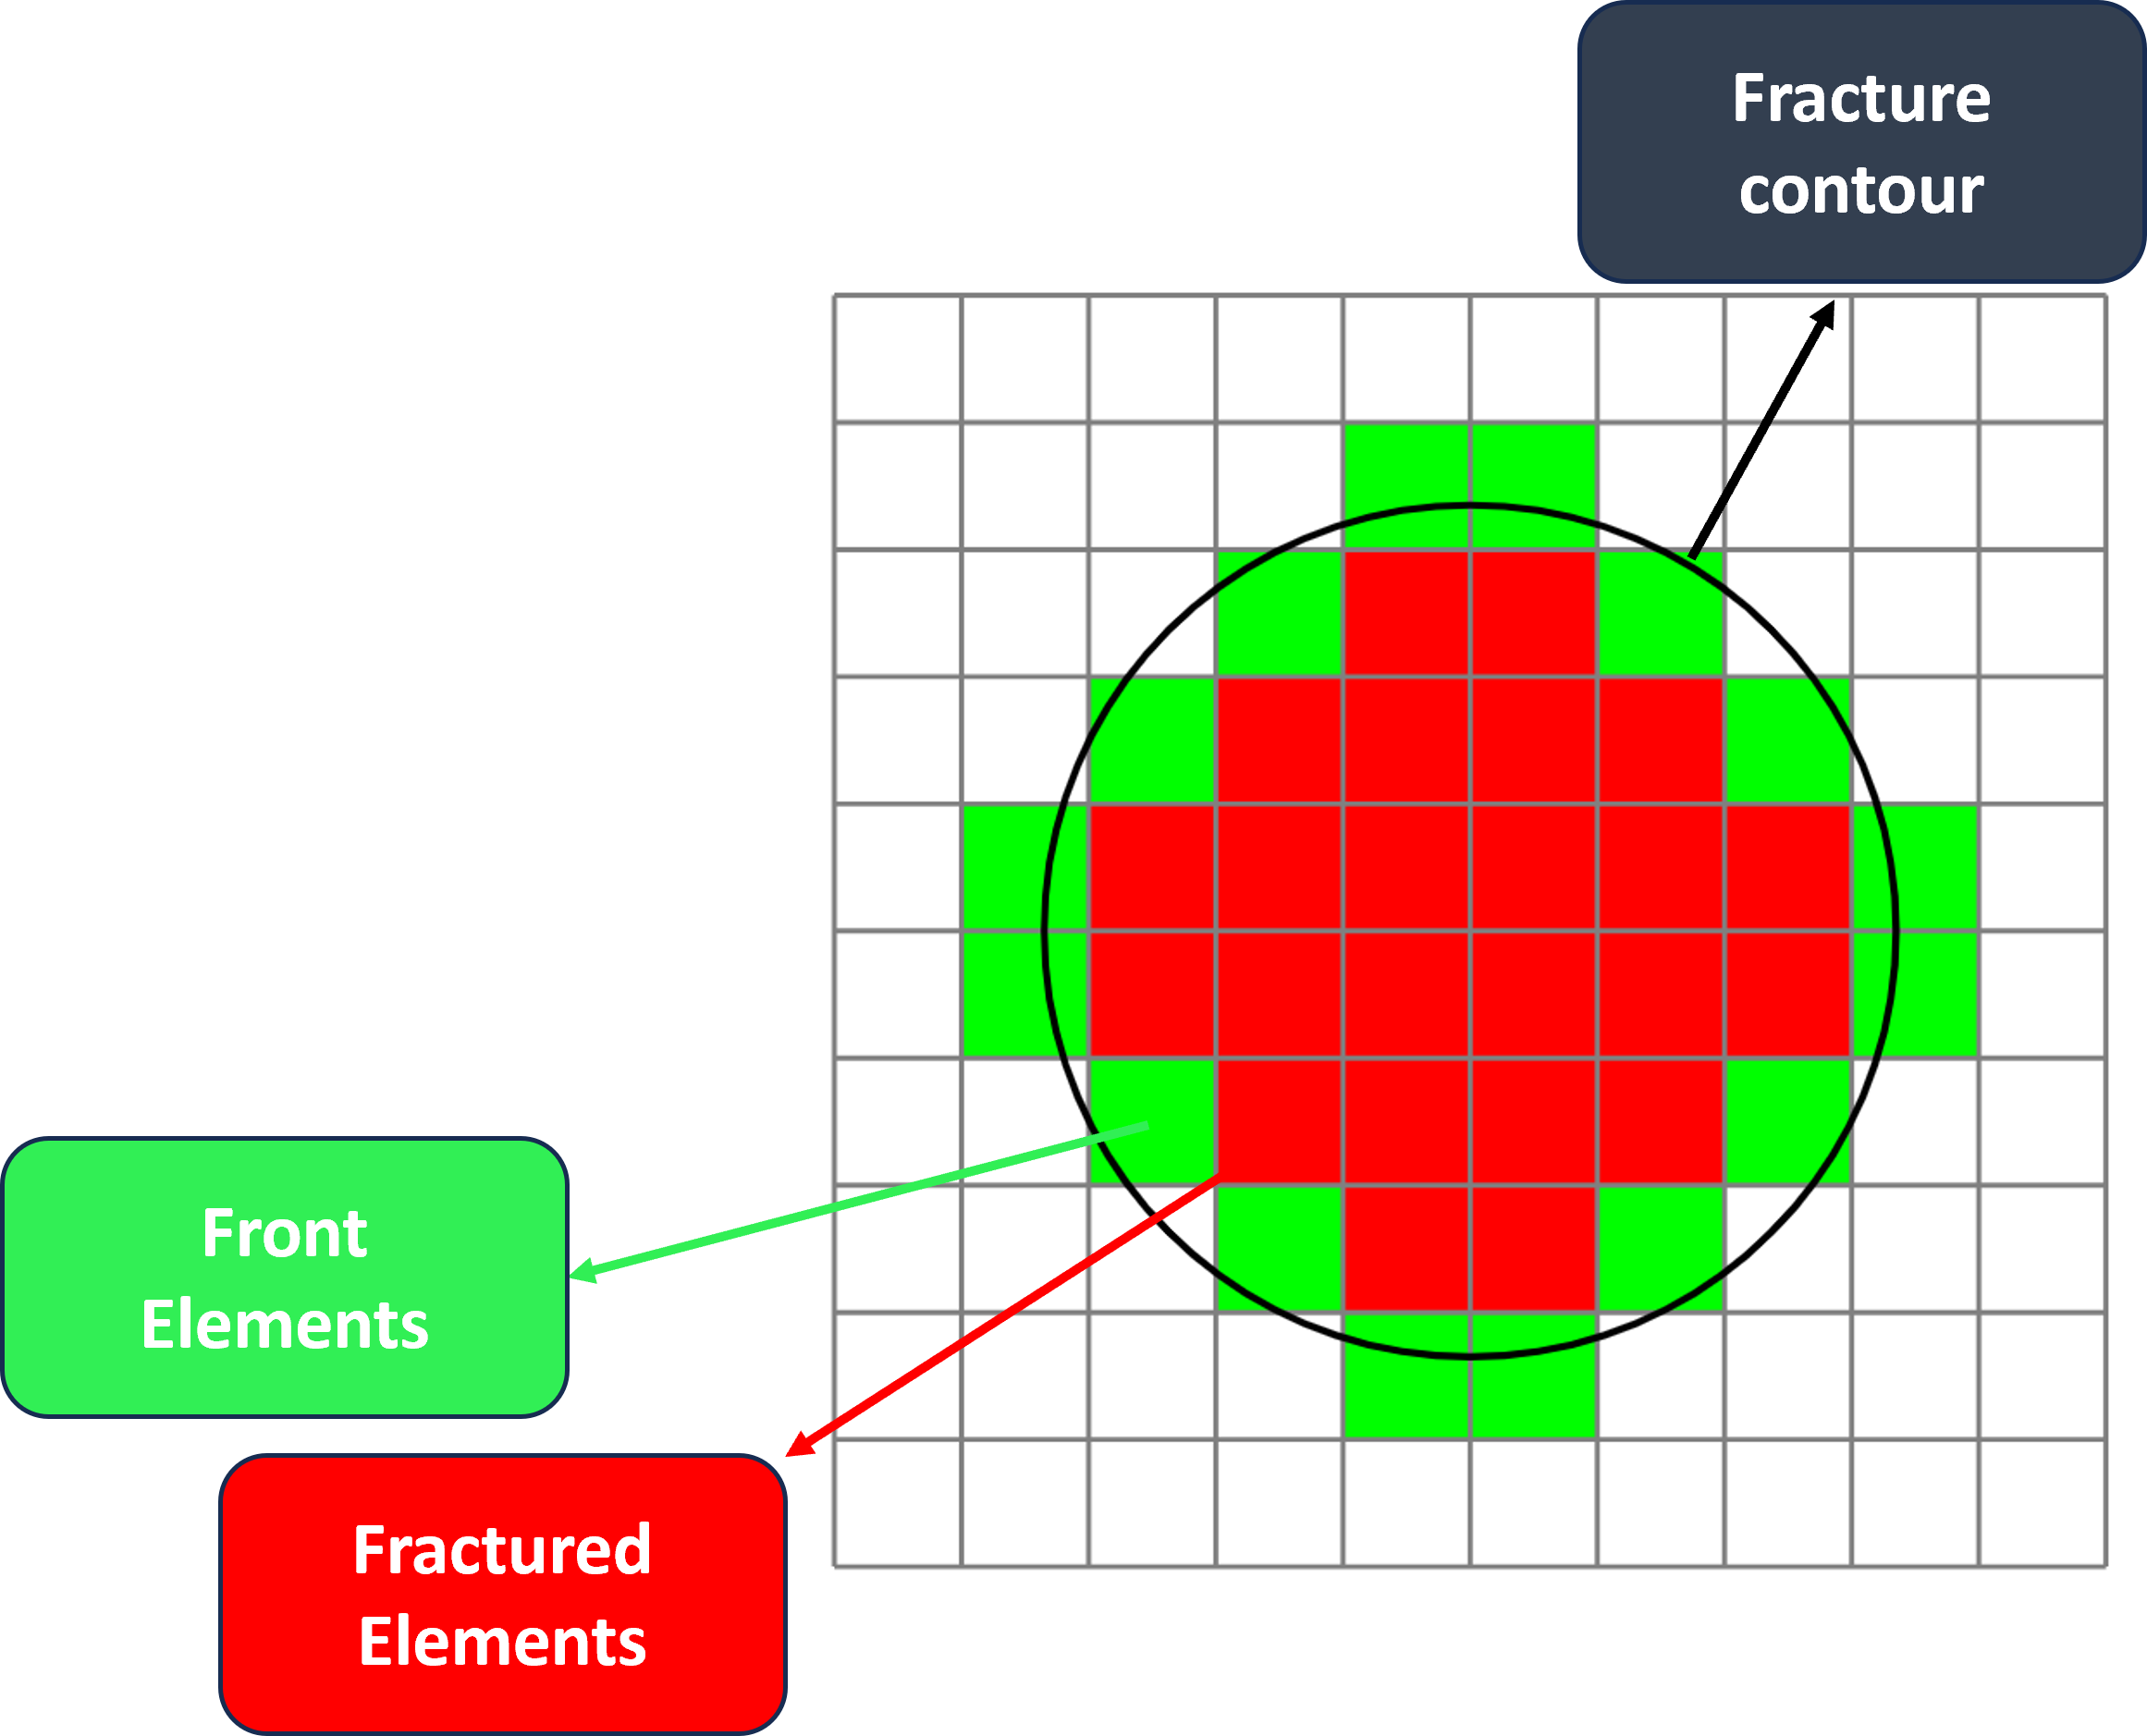
\includegraphics[width=\linewidth]{Chapter4/figures/penny_with_descriptions.png}
%         \caption{Multi-resolution solution algorithm.}
%         \label{fig:lorem1}
%     \end{subfigure}%
%     \bigskip
%     \begin{subfigure}{\textwidth}
%         \centering
%         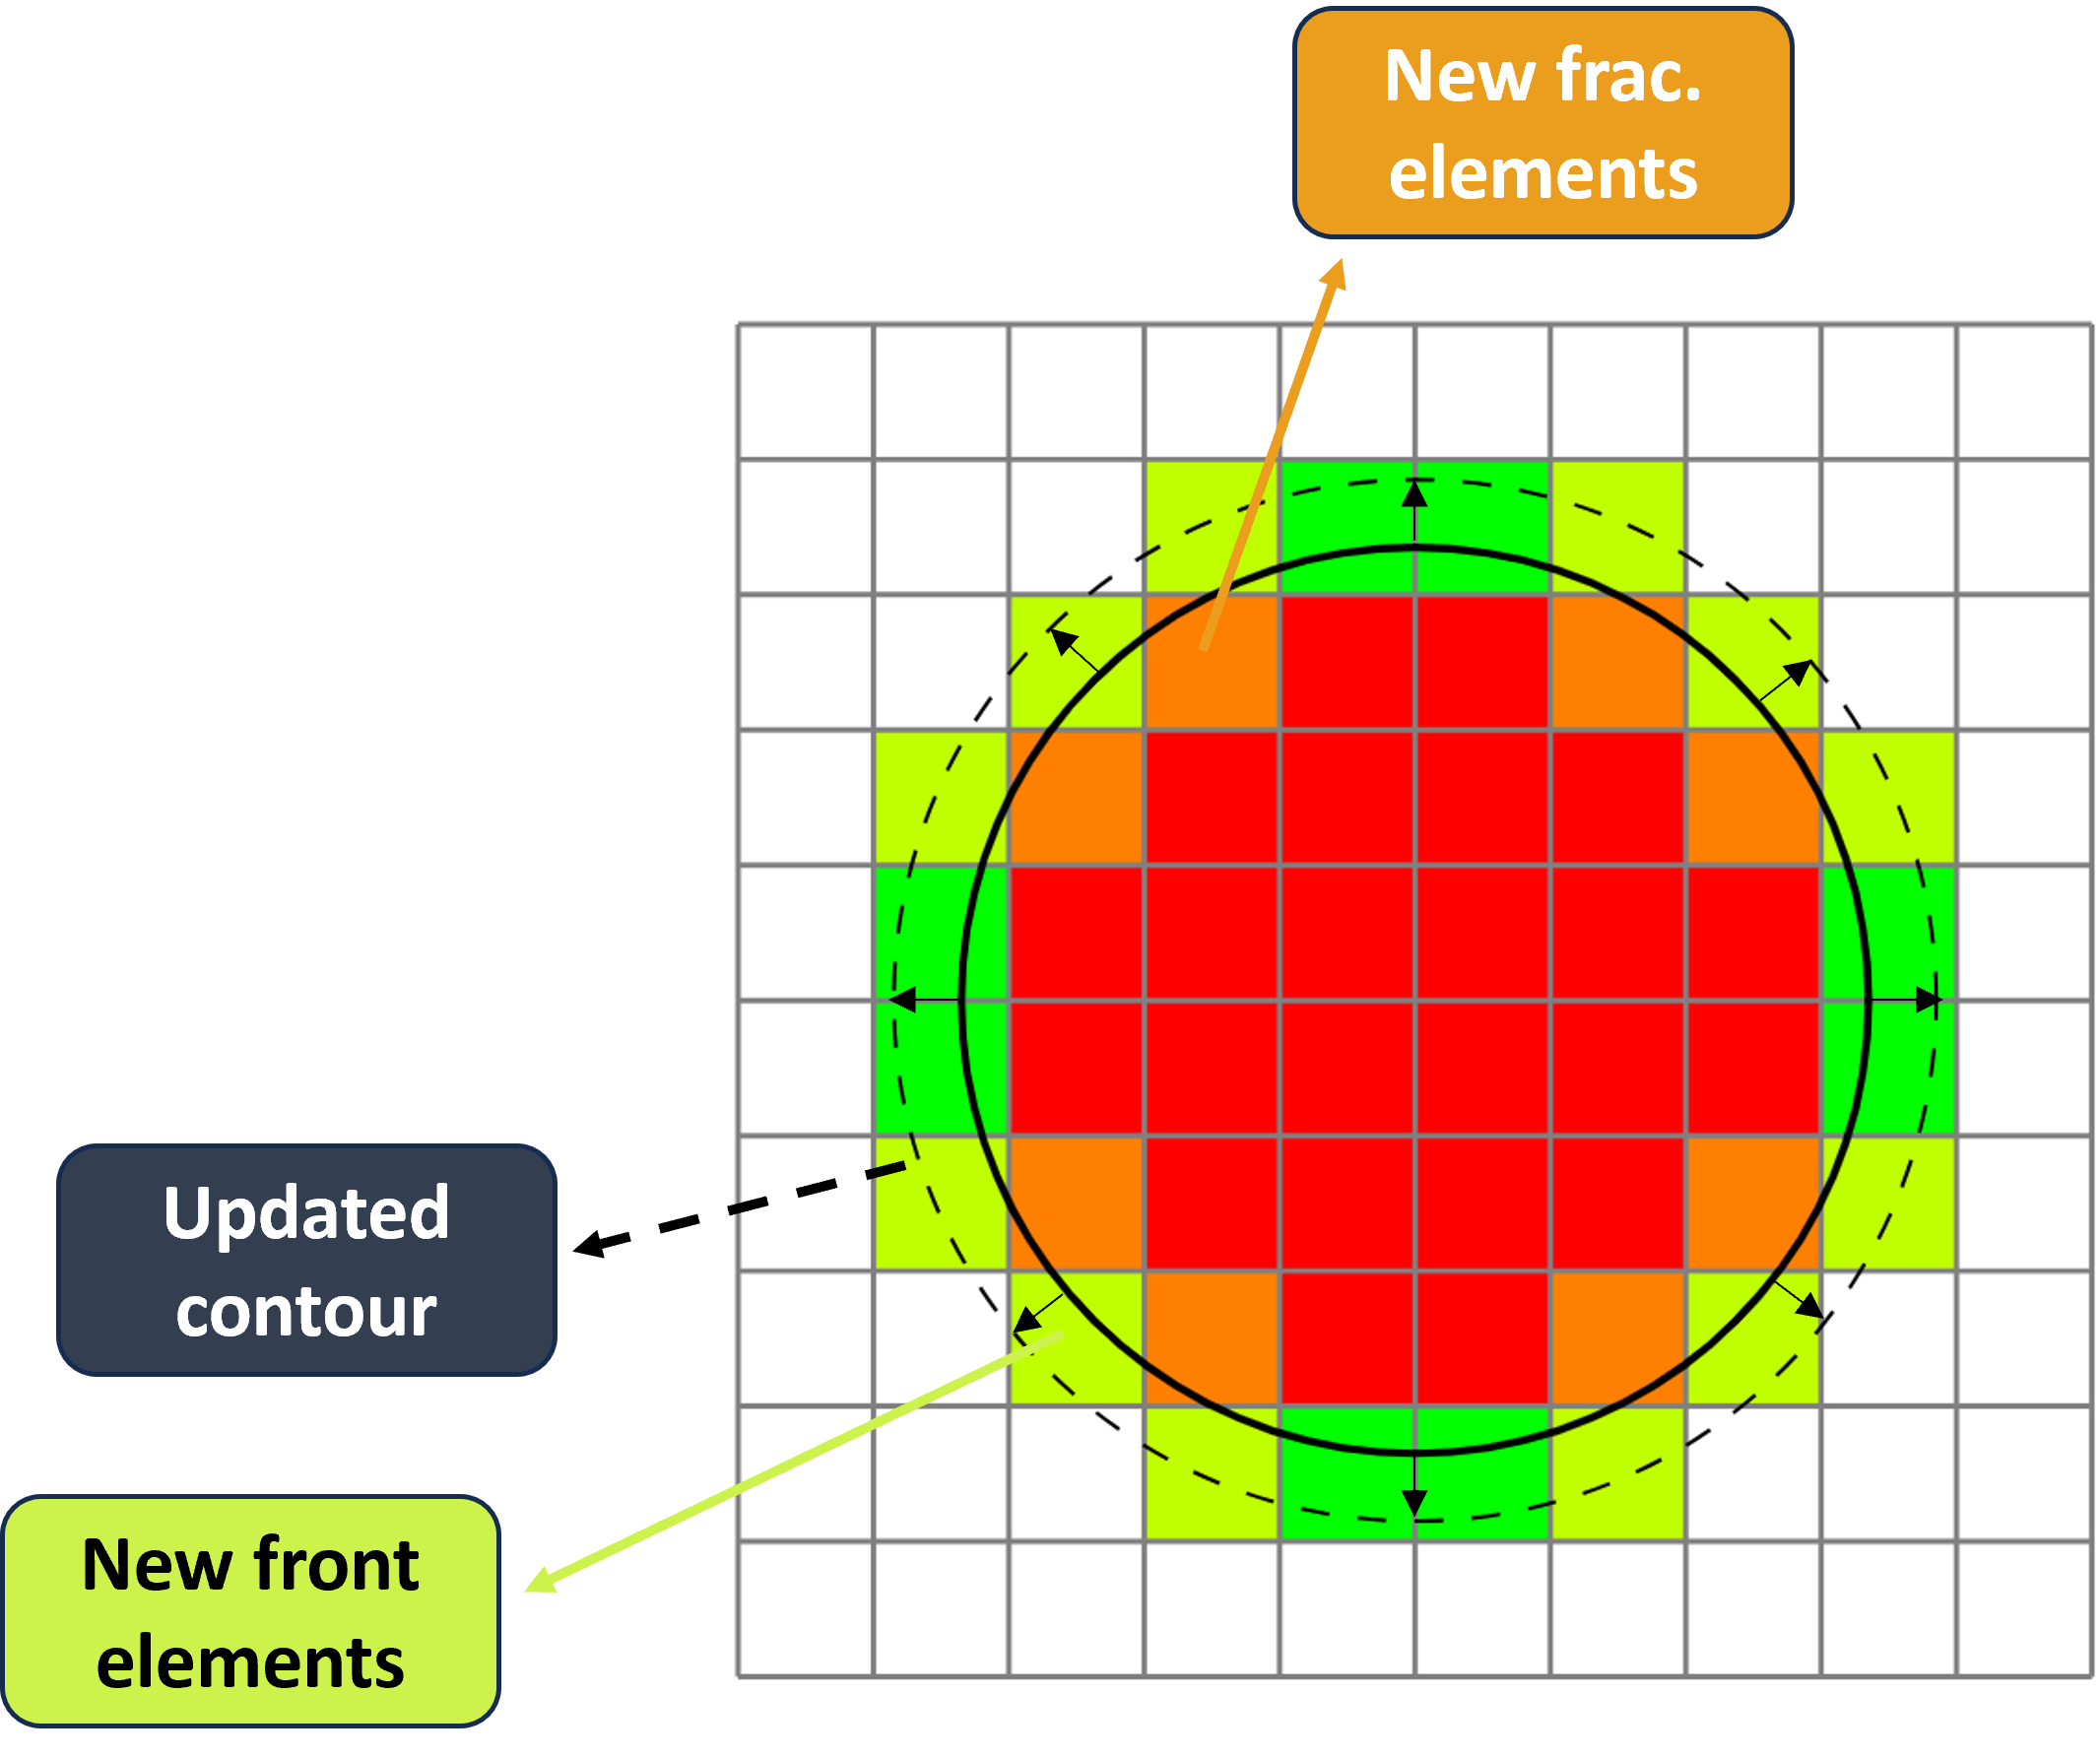
\includegraphics[width=\linewidth]{Chapter4/figures/larger_penny_with_descriptions.png}
%         \caption{Multi-resolution solution algorithm.}
%         \label{fig:lorem2}
%     \end{subfigure}
%     \bigskip
%     \begin{subfigure}{\textwidth}
%         \centering
%         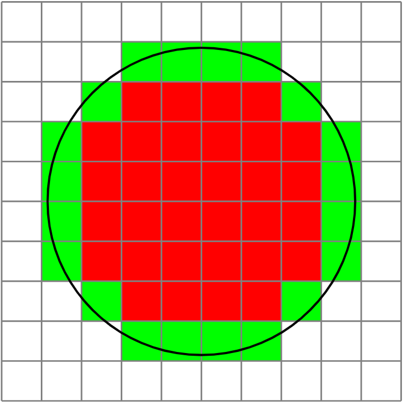
\includegraphics[width=0.65\linewidth]{Chapter4/figures/larger_penny.png}
%         \caption{Multi-resolution solution algorithm.}
%         \label{fig:lorem3}
%     \end{subfigure}
%     \caption{Schematic of propagation steps.}
% \end{figure}

\begin{figure}[h]
    \begin{subfigure}{\textwidth}
        \hspace*{1.85cm}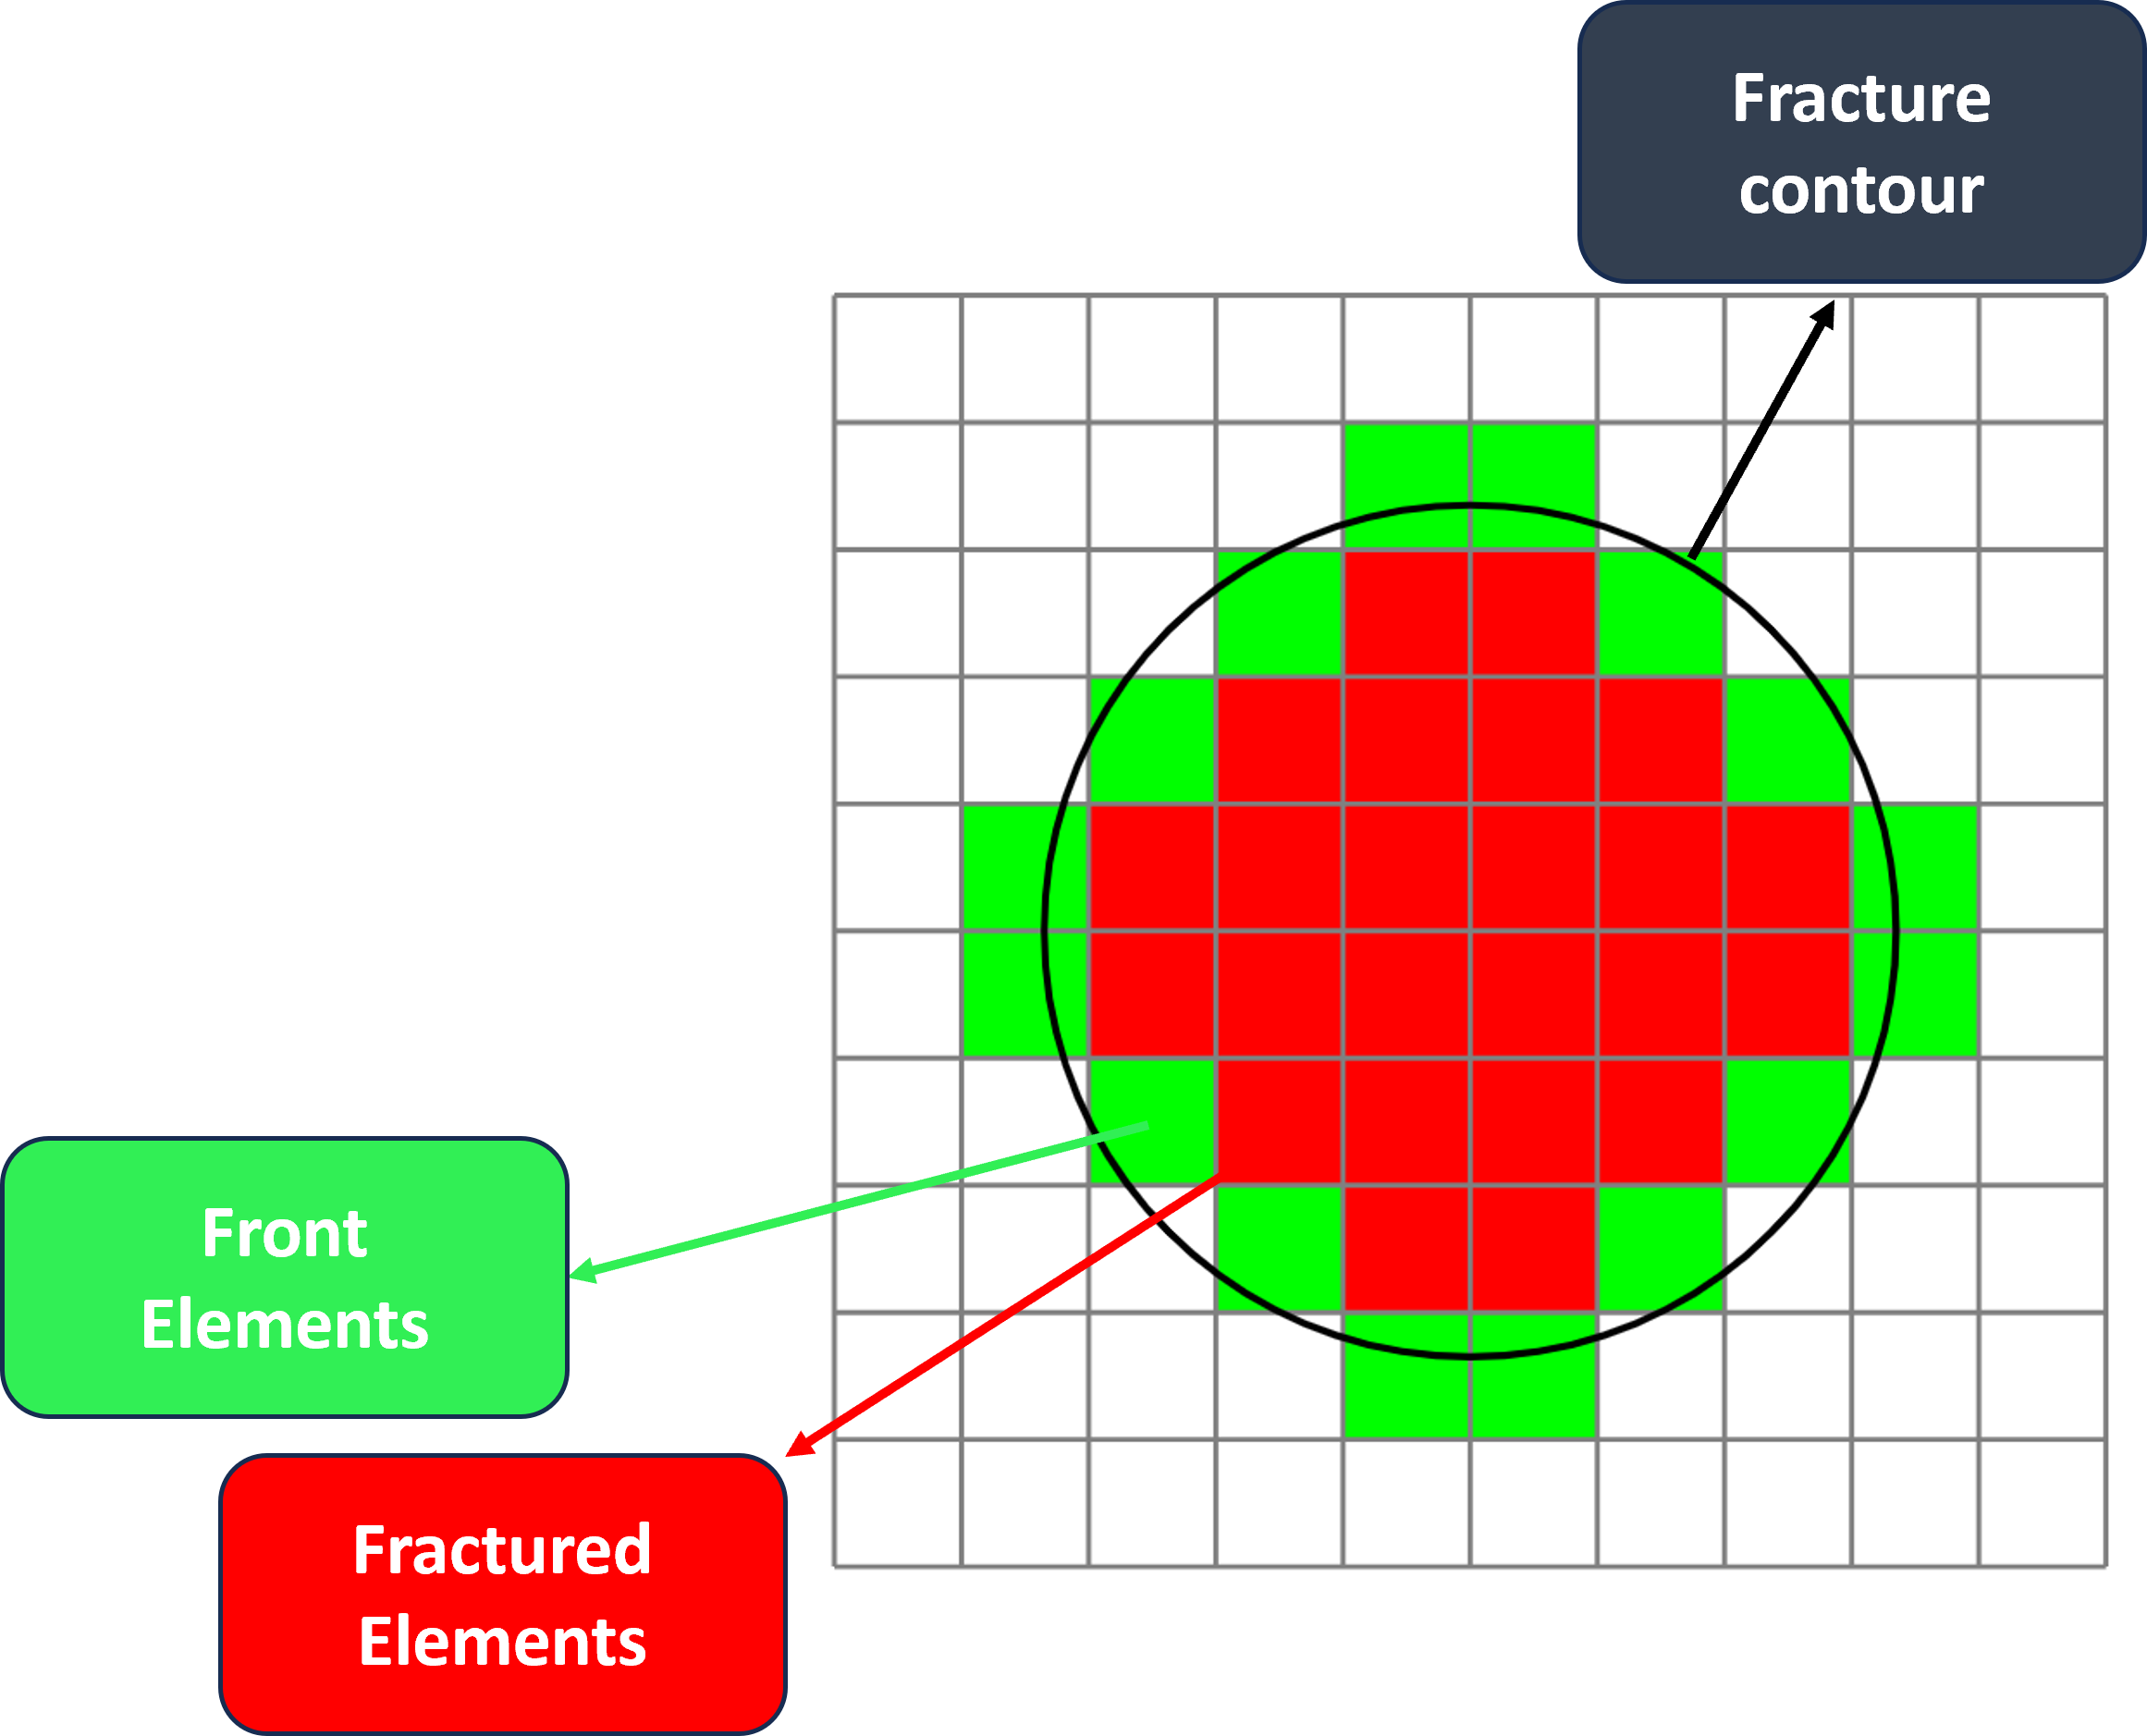
\includegraphics[width=0.55\linewidth]{Chapter4/figures/penny_with_descriptions.png}
        \caption{Initial state.}
        \label{fig:lorem1}
    \end{subfigure}

    \begin{subfigure}{\textwidth}    
        \hspace*{2.35cm}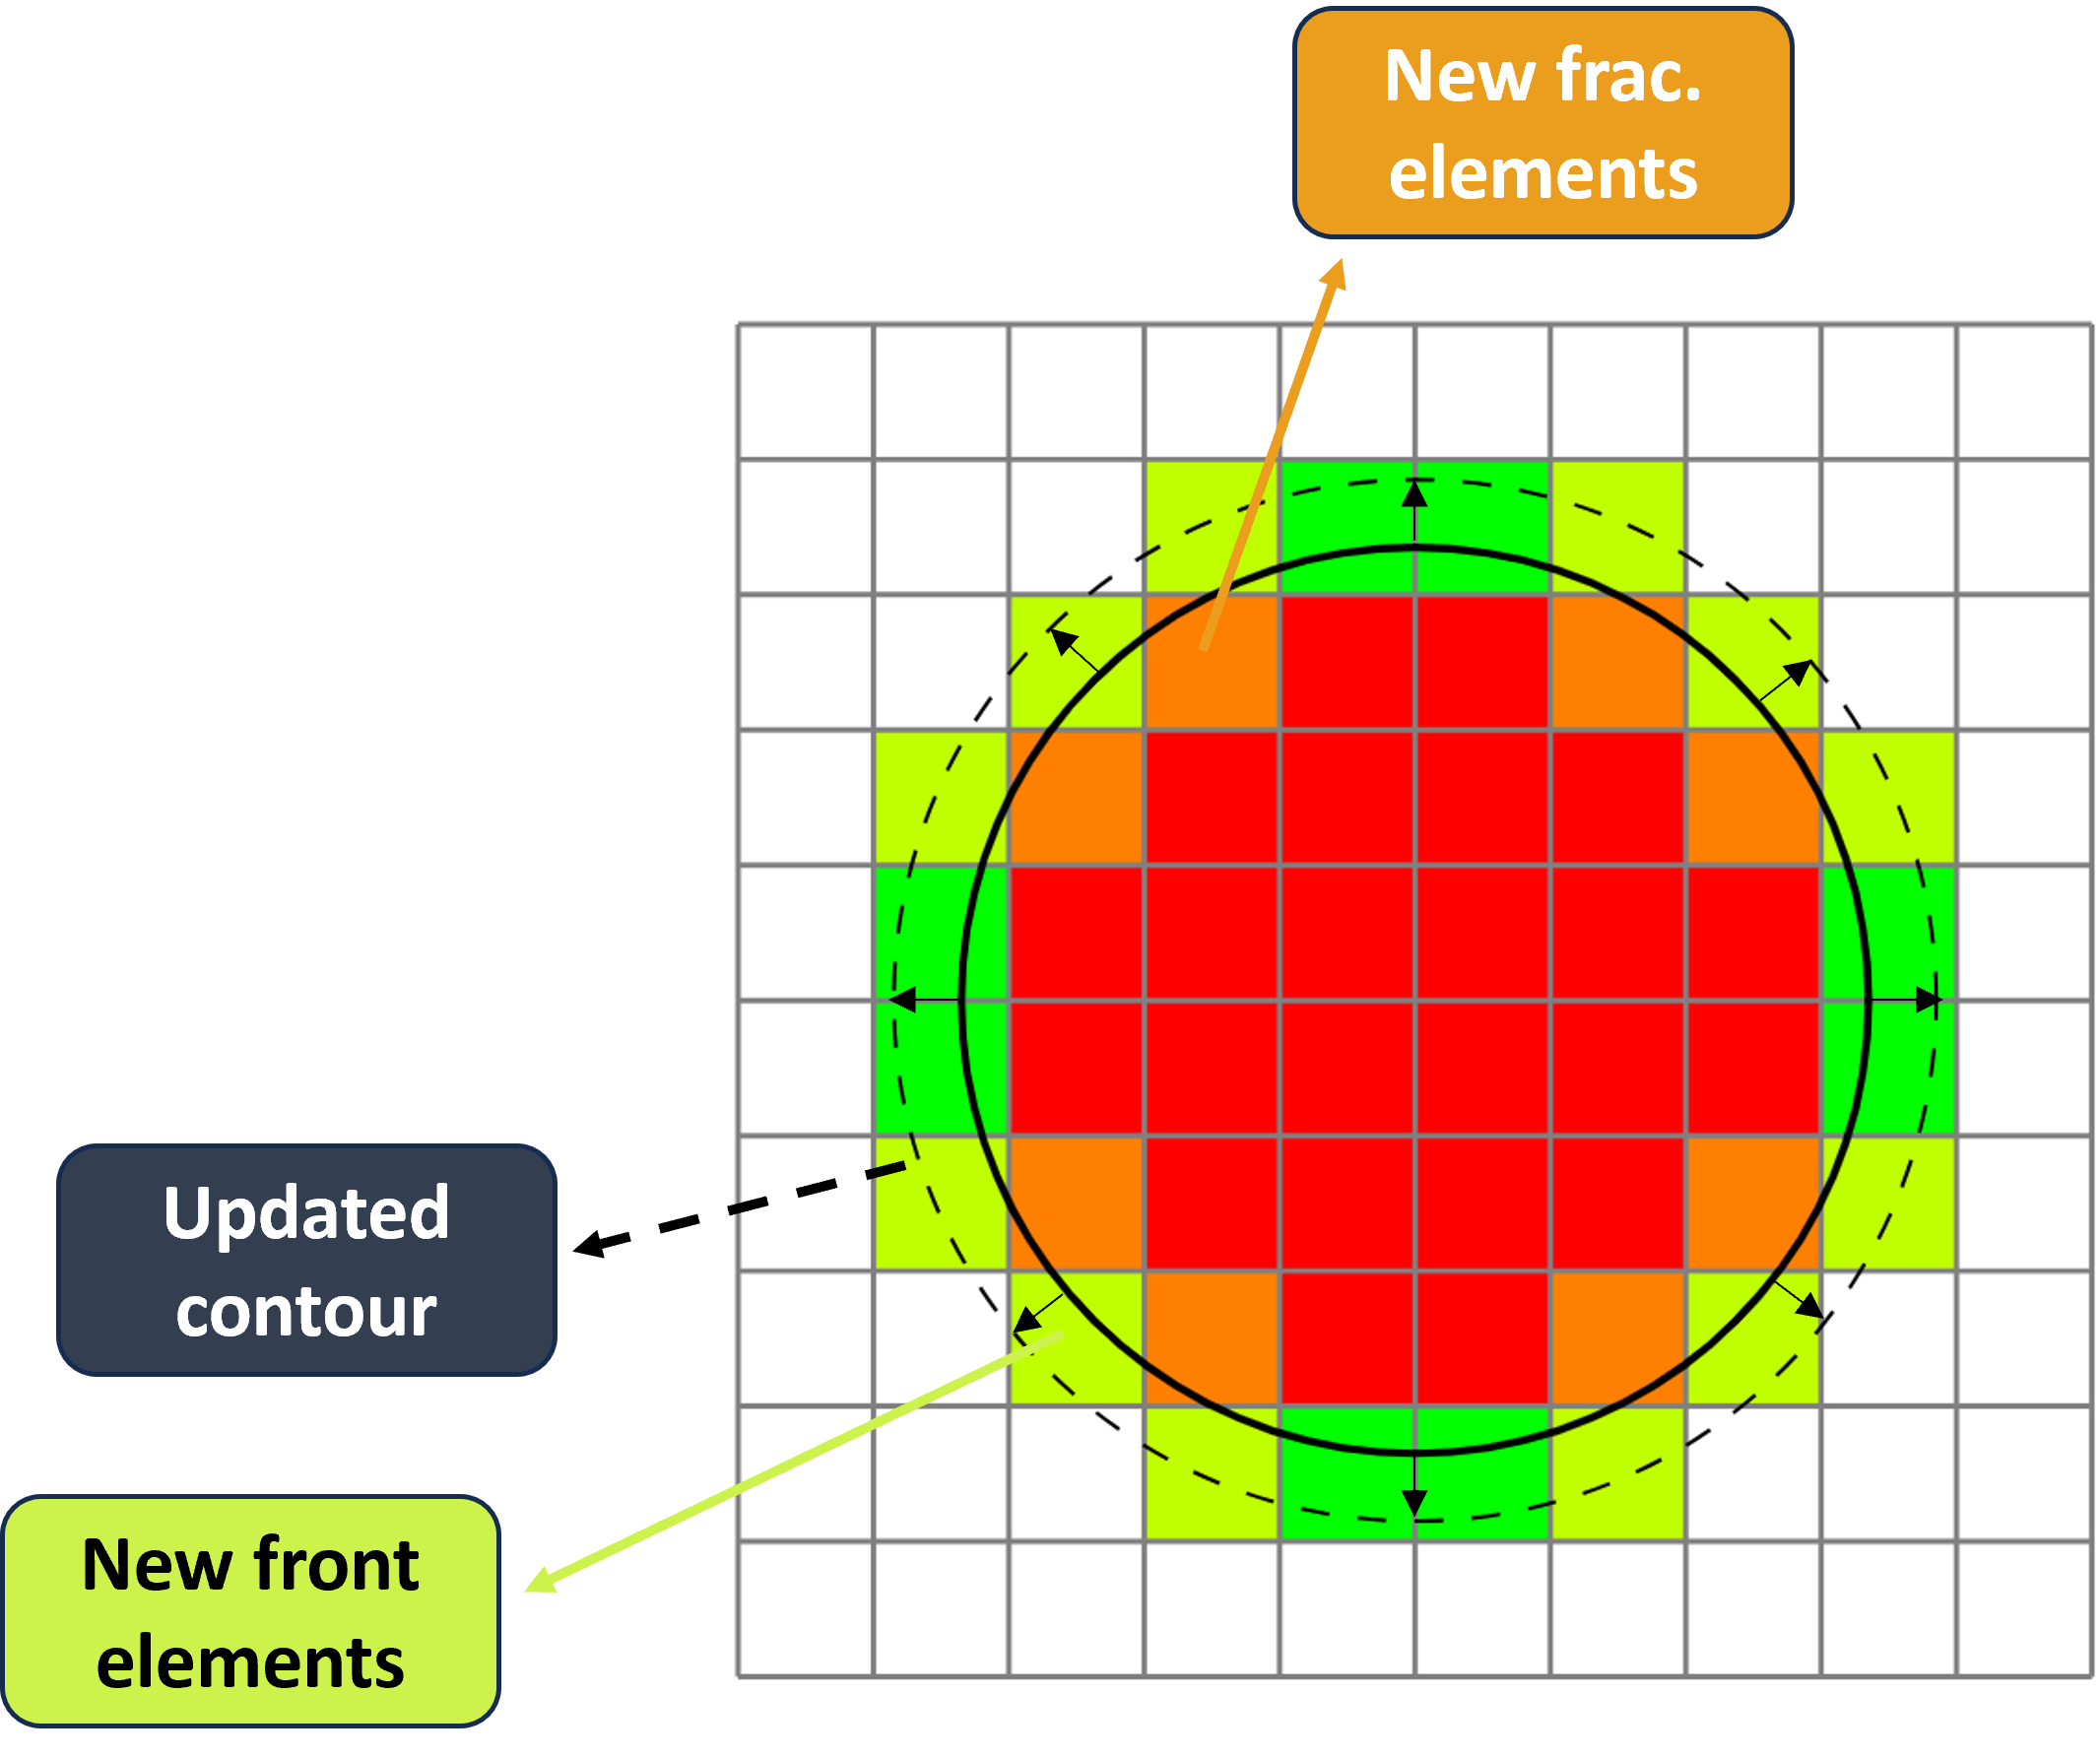
\includegraphics[width=0.51\linewidth]{Chapter4/figures/larger_penny_with_descriptions.png}
        \caption{Damage advanced.}
        \label{fig:lorem2}
    \end{subfigure}
    
    \begin{subfigure}{\textwidth}
        \centering
        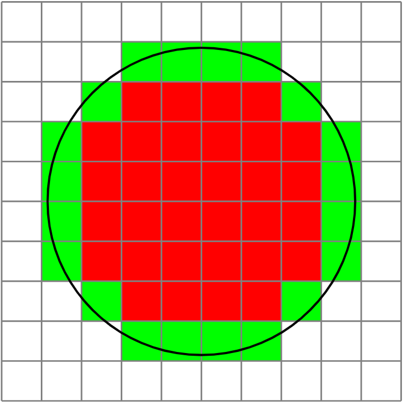
\includegraphics[width=0.33\linewidth]{Chapter4/figures/larger_penny.png}
        \caption{Updated configuration.}
        \label{fig:lorem3}
    \end{subfigure}
    \caption{Schematic of propagation steps.}
\end{figure}

